% =====================================================================
%  Prabhavit Gupta, one-page CV (Satispay - Software Engineer III, Backend - Consumer Wealth Domain)
%  Compile:  tectonic main_Satispay_SoftwareEngineerIII_Wealth.tex
%  Needs:    photo.jpg in the same folder as this .tex
%  Rules:    ONE PAGE. No em-dashes. Plain voice. Clickable companies.
% =====================================================================
\documentclass[a4paper,10pt]{article}

\usepackage[T1]{fontenc}
\usepackage[utf8]{inputenc}
\usepackage[top=0.75cm,bottom=0.75cm,left=1.0cm,right=1.0cm]{geometry}
\usepackage{titlesec}
\usepackage{enumitem}
\usepackage{hyperref}
\usepackage{xcolor}
\usepackage{graphicx}

\definecolor{accent}{HTML}{1F4E78}
\hypersetup{colorlinks=true, urlcolor=accent, linkcolor=accent}
\pagestyle{empty}
\setlength{\parindent}{0pt}

\titleformat{\section}{\large\bfseries\color{accent}}{}{0em}{}[\vspace{-0.6em}\rule{\textwidth}{0.8pt}]
\titlespacing{\section}{0pt}{2pt}{1pt}

\newcommand{\role}[4]{%
 \textbf{#1} \hfill \textbf{#2}\\[1pt]%
 \textit{#3} \hfill \textit{#4}\\[2pt]%
}
\setlist[itemize]{leftmargin=1.2em, itemsep=0pt, topsep=1pt, parsep=0pt}

\begin{document}

% ================= HEADER =================
\begin{minipage}[c]{0.80\textwidth}
 {\Huge\bfseries Prabhavit Gupta}\\[3pt]
 {\color{accent}\large Software Engineer III, Backend -- Consumer Wealth Domain}\\[6pt]
 {\footnotesize +39 351 610 7807 ~$\vert$~
 \href{mailto:prabhavitg@gmail.com}{prabhavitg@gmail.com} ~$\vert$~
 \href{https://www.linkedin.com/in/prabhavit/}{linkedin.com/in/prabhavit} ~$\vert$~
 \href{https://github.com/prab-gupta}{github.com/prab-gupta} ~$\vert$~
 Venice / Milan, Italy}
\end{minipage}\hfill
\begin{minipage}[c]{0.18\textwidth}
 \raggedleft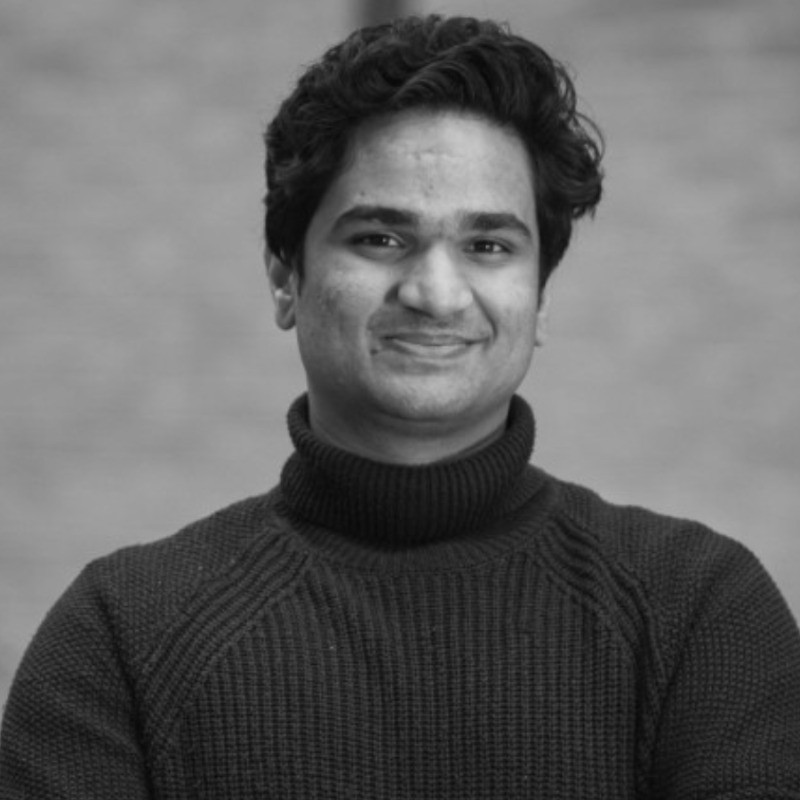
\includegraphics[width=2.0cm]{photo.jpg}
\end{minipage}
\vspace{-2pt}

% ================= SUMMARY =================
\section{Summary}
Product-minded Backend Engineer with over 3 years of experience architecting and operating scalable, high-reliability microservices and API engines. Adept at turning complex financial and business requirements into resilient technical solutions using modern cloud environments and relational databases like PostgreSQL. Passionate about system reliability, data integrity, and leveraging AI-powered development tools to elevate engineering speed and root-cause analysis. Proven track record of owning the full feature lifecycle and driving cross-functional delivery in fast-paced environments. 

% ================= SKILLS =================
\section{Skills}
\begin{itemize}
 \item \textbf{Backend \& Architecture:} Microservices architecture, RESTful APIs, OpenAPI contracts, webhooks, system reliability, transactional consistency, event-driven integrations
 \item \textbf{Languages \& Frameworks:} TypeScript, Node.js, Python (FastAPI, data pipelines), PHP (Laravel), SQL, Next.js
 \item \textbf{Cloud \& Infrastructure (AWS):} Cloud deployments, Docker, CI/CD, scalable product architecture, uptime monitoring, latency optimization
 \item \textbf{Databases:} PostgreSQL, Supabase, database schema design, entity pipelines, strict schema validation
 \item \textbf{AI-Powered Engineering:} Advanced utilization of LLMs and AI coding assistants for rapid root cause analysis, code optimization, testing, and documentation generation
\end{itemize}

% ================= EXPERIENCE =================
\section{Experience}

\role{\href{https://flowspace.co}{FlowSpace.co}}{Mar 2024 - Aug 2026}{Lead Developer \& Backend Engineer (Full-time, Freelance)}{London, UK (Remote)}
\begin{itemize}
 \item Led the core platform migration off a legacy stack to a coded Next.js and Laravel architecture, designing resilient database schemas and entity pipelines in PostgreSQL while scaling users from 2,000 to 4,500+.
 \item Engineered and operated production REST APIs and webhooks integrating third-party platforms with robust schema validation, error handling, and uptime monitoring for high reliability.
 \item Architected and deployed an end-to-end multi-agent AI ingestion pipeline extracting structured data from unstructured multi-format sources, enforcing strict data integrity.
 \item Deployed conversational support agents querying live platform records, implementing deterministic fallback paths to human operators for fail-safe service.
 \item Defined development workflows, CI/CD test automation, and engineering standards, extensively leveraging AI-powered tools to optimize code delivery and maintain system health.
\end{itemize}

\role{\href{https://ultrastrategy.com}{UltraStrategy.com}}{Dec 2024 - May 2025}{Backend Automation Developer (Collaborator)}{France (Remote)}
\begin{itemize}
 \item Developed a high-throughput data-processing pipeline using workflow automation and AI integrations, converting unstructured data into standardized relational schemas across diverse profiles.
\end{itemize}

\role{Urlink}{Apr 2025 - Jul 2025}{Project Manager \& AI-Assisted Developer (Freelance)}{Barcelona, Spain (Remote)}
\begin{itemize}
 \item Directed technical requirements and built backend application logic, database structures, and client automations with a strong focus on AI-assisted development tools. Stack: Next.js, Supabase (PostgreSQL).
\end{itemize}

\role{\href{https://get2germany.com}{Get2Germany.com}}{Jan 2024 - May 2024}{Backend Developer \& Automation Specialist (Part-time)}{Berlin, Germany (Remote)}
\begin{itemize}
 \item Built automated ETL pipelines integrating external APIs and custom workflows to aggregate, classify, and reliably serve complex domain data.
\end{itemize}

% ================= EDUCATION =================
\section{Education}
\textbf{Ca' Foscari University of Venice} \hfill Oct 2020 - Jun 2024\\
BA Philosophy, International Studies \& Economics (Minor: Entrepreneurship) \hfill Venice, Italy\\
{\footnotesize Core focus: Analytical logic, quantitative decision theory, economic modeling, and technology innovation.}

% ================= WORK AUTH =================
\vspace{2pt}
{\small \textbf{Work Authorization:} European Long Term Residence Permit (Italy); full Italian and EU work rights with zero sponsorship required. \quad \textbf{Languages:} English (fluent C2), Italian (conversational), Hindi (native).}

\end{document}
